
\newcommand{\vdmkw}[1]{\texttt{\textbf{#1}}}
\chapter{Automatic Generation of Code}\label{sec:codegen}

It is possible to generate Java code\index{code generation} for a
large subset of VDM-SL and VDM++ models. In addition to Java, C and
C++ code generators are currently being developed. Both these code
generators are in the early stages of development. For
comparison, code generation of VDM-SL and VDM++ specifications to both
Java and C++ is a feature that is available in
VDMTools~\cite{Java2VDMMan,CGMan,CGManPP}. The majority of this
chapter focuses solely on the Java code generator available in
VDM VSCode Extension.

\section{Use of the Java Code Generator}
\label{sec:javacg_use}

\begin{figure}[htbp]
\begin{center}
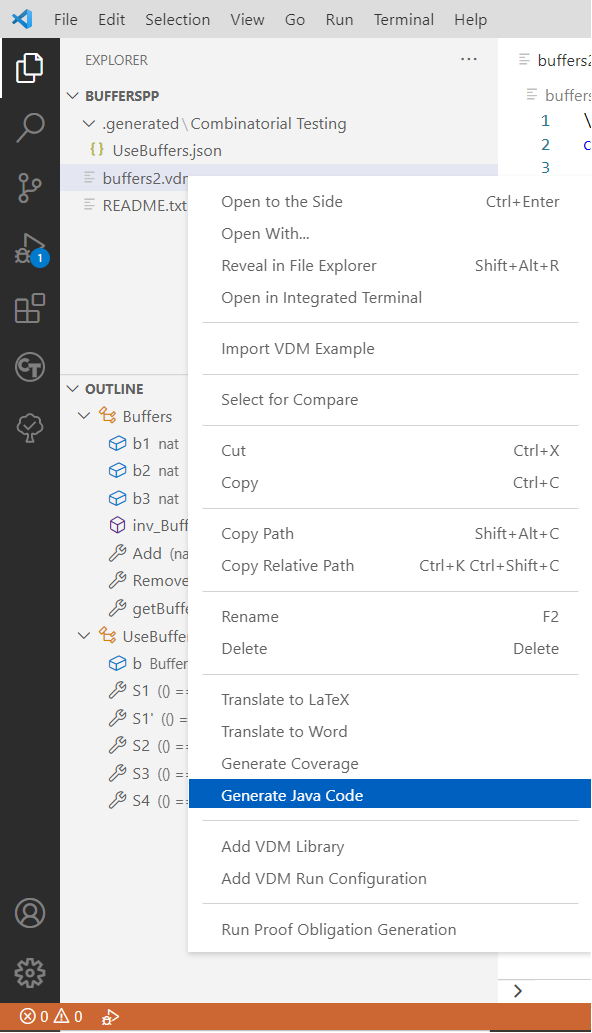
\includegraphics[width=10cm]{snapshots/Launching the java code generator.png}
\caption{Launching the Java code generator.\label{fig:javacg_menu}}
\end{center}
\end{figure}

\begin{figure}[htbp]
\begin{center}
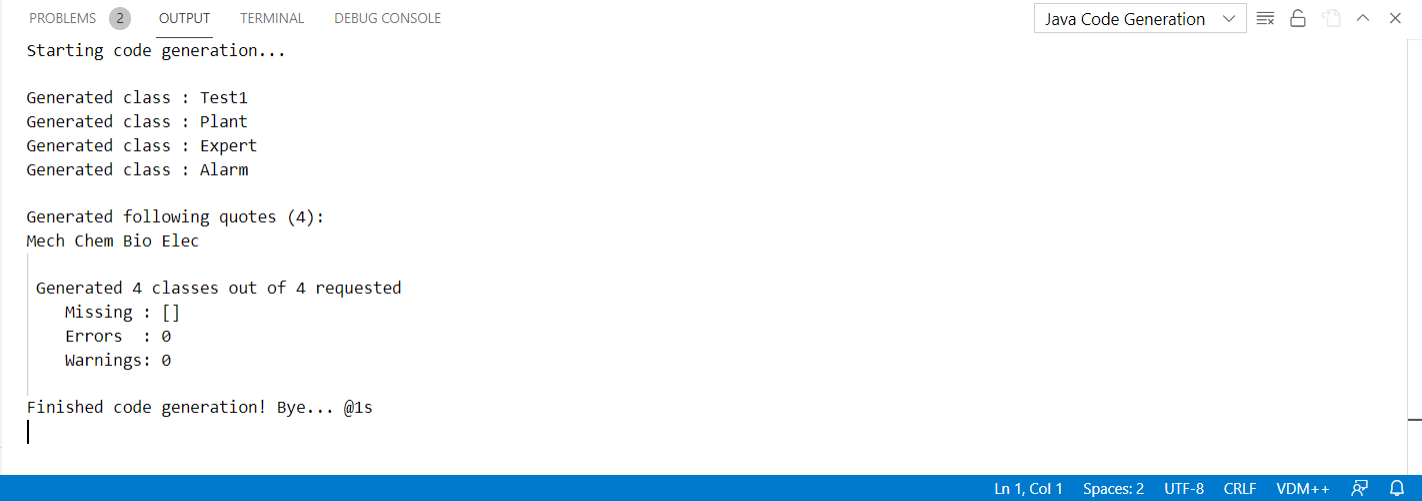
\includegraphics[width=\linewidth]{snapshots/Status of code generating the Alarm PP example.png}
\caption{The status of code generating the \texttt{AlarmPP}
example.\label{fig:javacg_output}}
\end{center}
\end{figure}

The Java code generator can be launched via the context menu as shown
in Figure~\ref{fig:javacg_menu}. Alternatively, this can be done by
highlighting the project in the VDM Explorer and typing one of the
shortcuts associated to this plugin. To launch the Java Code Generation, right click on file and select 'Generate Java Code'.\\


\noindent Upon completion of the code generation process the status is
output to the console as shown in Figure~\ref{fig:javacg_output}. In
particular this figure shows the status of code generating the
\texttt{AlarmPP} model available in the Overture standard examples. As
indicated by the console output, the generated code is available as an
VSCode project in the \texttt{generated/java}
folder.




\section{Limitations of the Java Code Generator}

If the Java code generator encounters a construct that it cannot code
generate it will report it as unsupported to the user and the user can
then try to rewrite that part of the specification using other
(supported) constructs. Reporting of unsupported constructs is done
via the console output and using editor markers.\\

\clearpage
The user will get similar messages and markers for other unsupported
VDM constructs. To summarise, the Java code generator currently does
not support code generation of multiple inheritance and neither does
it support traces, type binds, invariant checks and pre and post
conditions. Furthermore, let expressions appearing on the right-hand
side of an assignment will also be reported as unsupported. The Java
code generator also does not support every pattern. The patterns that
are currently not supported are: object, map union, map, union, set,
sequence, concatenation and match value.

\section{The Code Generation Runtime Library}

The generated code relies on a runtime library used to represent some
of the types available in VDM (tokens, tuples etc.) as well as
collections and support for some of the complex operators such as
sequence modifications. For simplicity every project generated
by the Java code generator contains the runtime library. More
specifically, there is a copy of the runtime library containing only
the binaries (\texttt{lib/codegen-runtime.jar}) as well as a version
of the runtime library that has the source code attached
(\texttt{lib/codegen-runtime-sources.jar}). The runtime library is
imported by every code generated class using the Java import statement
\texttt{\textbf{import} org.overture.codegen.runtime.*;} and in order
to compile the generated Java code the runtime library must be visible
to the Java compiler.

Similar to VDMTools the runtime library also provides implementation
for subset of the functionality available in the standard libraries:
The runtime library provides a full implementation of the
\texttt{MATH} library, support for conversion of values into character
sequences as provided by the \texttt{VDMUtil}, and finally
functionality to write to the console as available in the \texttt{IO}
library.

\section{Configuration of the Java Code Generator}

The Java code generator can be configured via a preference page as shown in Figure~\ref{fig:javaGenerationConfiguration}. The
preference page can be accessed by :
\begin{enumerate}
    \item Clicking on 'File' (left top corner), select 'Preferences', then Settings
    \item Choosing 'Workspace' (not 'User')
    \item Going below in 'Extensions' and 'VDM VSCode'
\end{enumerate}
See Figure~\ref{fig:pathVDMSettings1} for more details

\begin{figure}[htbp]
\begin{center}
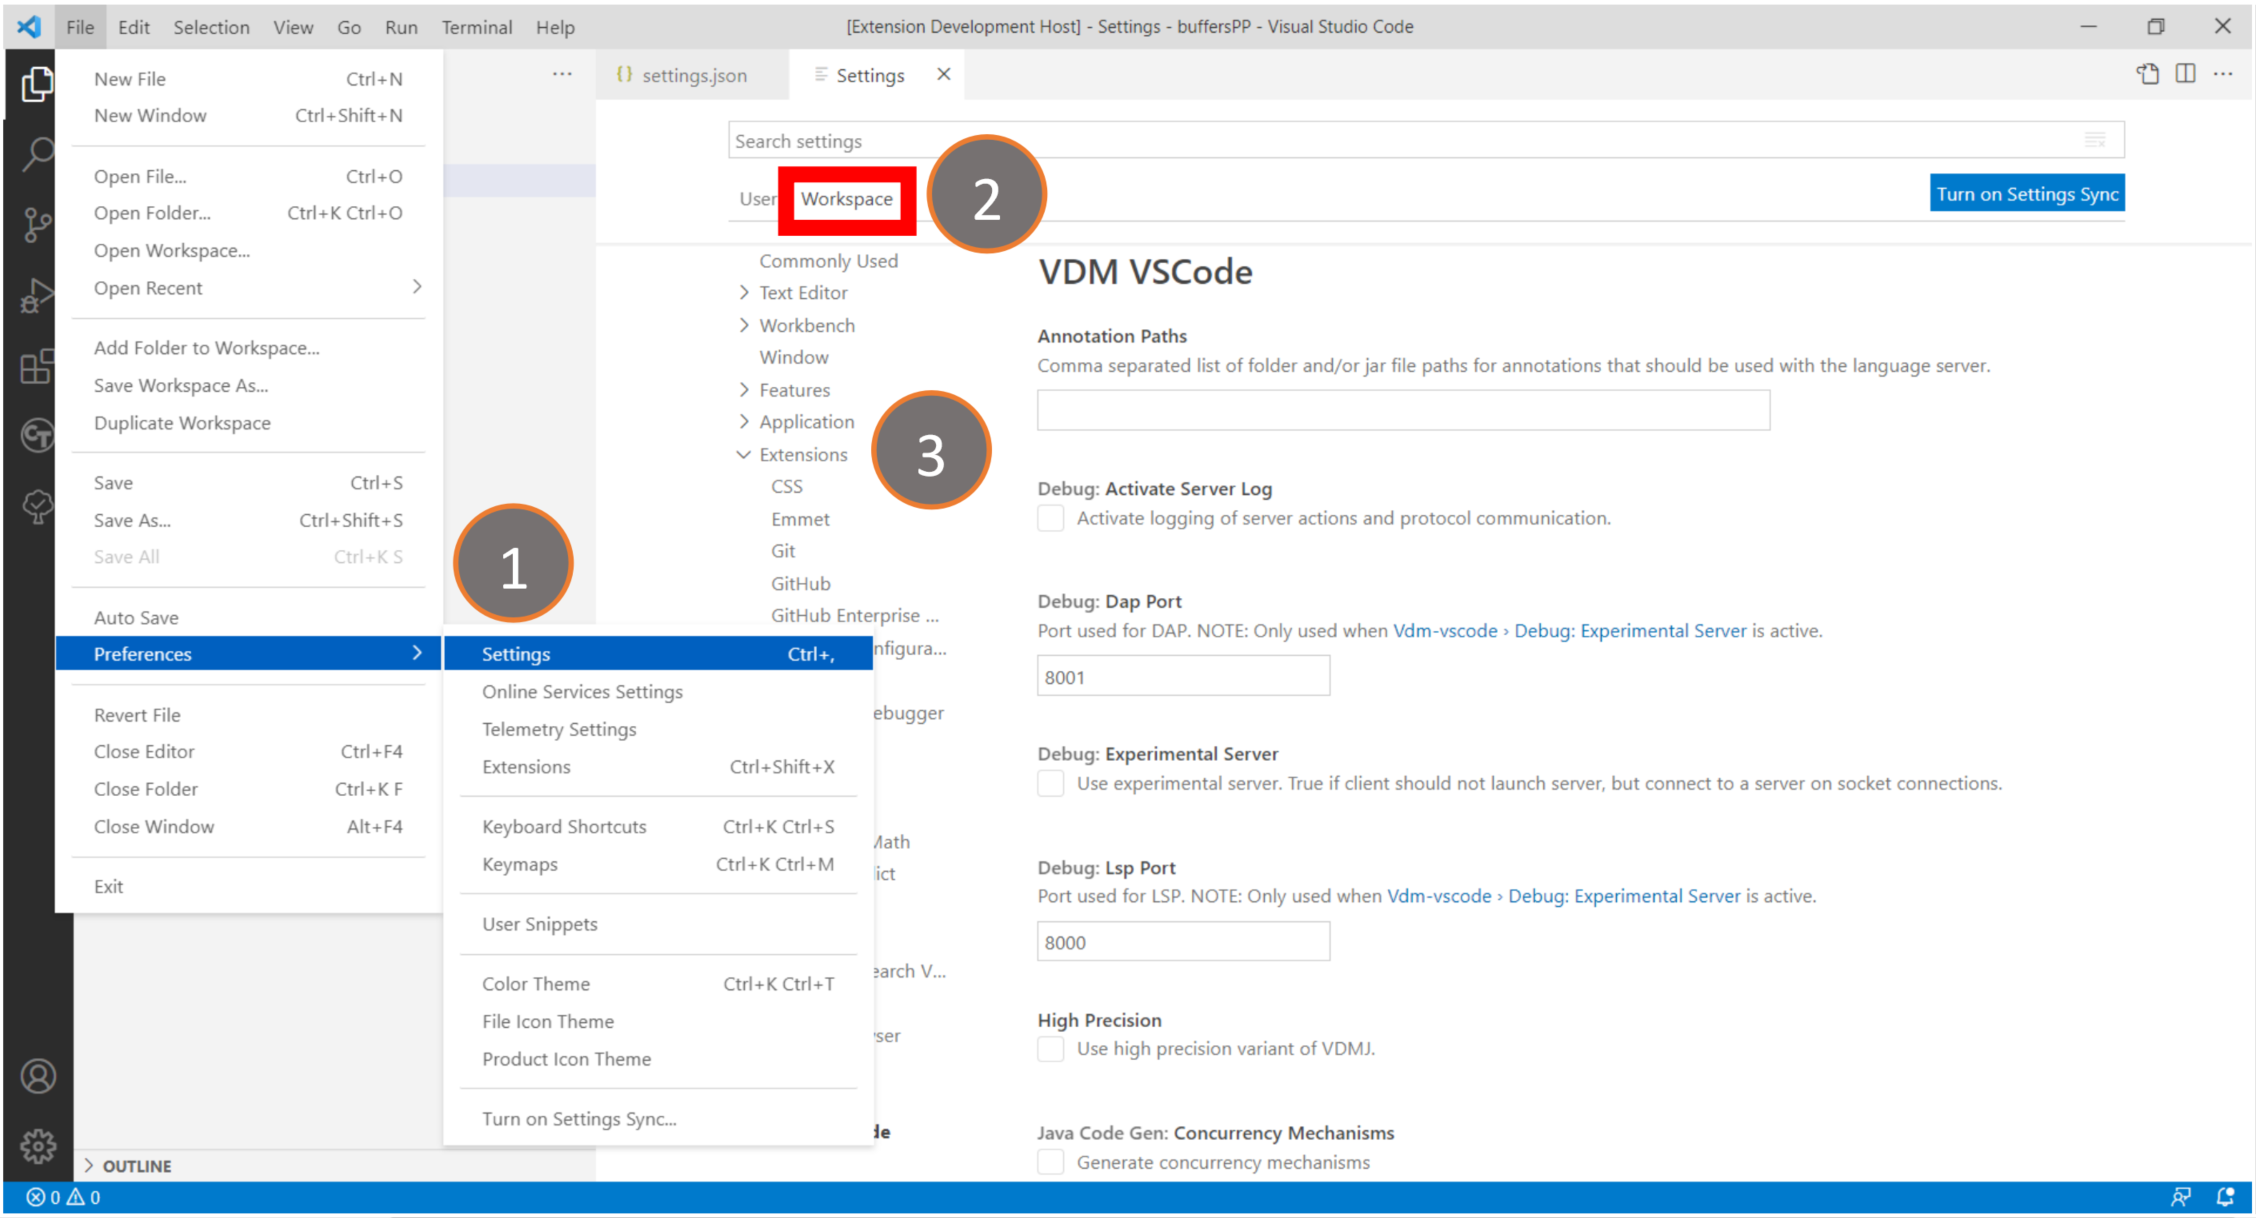
\includegraphics[width=16cm]{snapshots/Path to go to VDM settings.PNG}
\caption{Path to go to Java Code Configuration\label{fig:pathVDMSettings1}}
\end{center}
\end{figure}

\begin{figure}[htbp]
\begin{center}
\includegraphics[width=16cm]{snapshots/Settings for java code generation.png}
\caption{Configuration of the Java Code Generator\label{fig:javaGenerationConfiguration}}
\end{center}
\end{figure}

\newpage
The Java code generator provides a few options that allows the user to configure the code generation process (see Figure~\ref{fig:javaGenerationConfiguration}). The subsections
below treat each of these configuration parameters individually, in the order they appear
in the preference page.

\subsection{Disable cloning}
In order to respect the value semantics of VDM the Java code generator sometime needs to perform
deep copying of objects that represent composite value types (records, tuples, tokens, sets,
sequences and maps). For example, in VDM a record is a value type, which means that occurrences
of the record must be copied when it appears in the right-hand side of an assignment, it is passed
as an argument or returned as a result. However, Java does not support composite value types like
structs and records, and as a consequence record types must be represented using classes, which
use reference semantics. This means that an object reference, which is used to represent a composite
value type in the generated Java code must be deep copied when it appears in the right-hand
side of an assignment, it is passed as an argument or returned as a result. For arbitrarily complex
value types (such as records composed of record) deep copying may
introduce a significant overhead in the generated code. If the specification subject to code generation
does not truly rely on value semantics the user may wish to disable deep copying of value
types in the generated code in order to remove this overhead. The user should, however, be aware
that disabling of cloning may lead to code being generated that does not preserve the semantics
of the input specification and in general disabling of cloning is discouraged. By default cloning is
enabled.

\subsection{Generate character sequences as strings}
In VDM a string is a sequence of characters and there is no notion of a string type. Java in particular
works differently since it uses a separate type to represent a string. The default behaviour of the
Java code generator is to code generate sequences of characters as strings and subsequently do
the necessary conversion between between strings and sequences in the generated code. Another
possibility is to treat a string literal for what it truly is, namely a sequence of characters, and
thereby avoid any conversion between strings and sequences. In order to do that, i.e. not generating
character sequences as strings, the corresponding option must be unchecked.

\subsection{Generate concurrency mechanisms}
If the user does not rely on the concurrency mechanisms of VDM++ and does not want to include
support for them in the generated code the corresponding option in the preference page must be
unchecked. By default the behaviour of the Java code generator is to not include support for the
concurrency mechanisms of VDM++ in the generated code.

\subsection{Generate VDM location information for code generated constructs}
When a VDM model is code generated it can be helpful to know where the constructs in the generated
code originate from. When this option is enabled the Java code generator will generate
VDM location information for methods, statements and local declarations in the generated code.
More specifically, the Java code generator will generate a Java source code comment containing
the name of the VDM source file and the line number and the position, for each method, statement
and local declaration. As an example, the code fragment below says that the Java return statement
originates from a VDM construct at line 25, position 12 in \texttt{File.vdmsl.\\
/* File.vdmsl 25:12 */\\
return 42;}

\subsection{Choose output package}
The Java code generator allows the output package of the generated code to be specified. If the
user does not specify a package, the code generator outputs the generated Java code to a package
with the same name as the VDM project. If the name of the project is not a valid java package,
then the generated code is output to the default Java package.

\subsection{Skip classes/modules during the code generation process}
It may not always make sense to code generate every class or module in a VDM project. A class
or module can often be skipped if it acts as an execution entry point or it is used to load input for
the specification. Classes or modules that the user wants to skip can be specified in the text box
in the Java code generator preference page by separating the class/module names by a semicolon.
As an example, \texttt{World;Env} makes the code generator skip code generation of \texttt{World} and \texttt{Env}, while generating code for any other module or class. For convenience the output of the Java code
generator will also inform the user about what classes or modules are being skipped.

\newpage
\section{Translation of the VDM types and type constructors}
\label{sec:type-mappings}

Table ~\ref{tbl:type-mappings} describes how the VDM type(s) in the
left column are represented in the generated Java code (the right
column). In this table \texttt{pack} is the user-specified root
package of the generated Java code
and \texttt{E}, \texttt{D} and \texttt{R} represent arbitrary VDM
types. The type mapping in the last row is only used when the
\emph{Generate character sequences as strings} option is selected. Some of the types used to represent the VDM types are native Java types (from package
\texttt{java.lang}), others are part of the Java code generator
runtime library (from package \texttt{org.overture.codegen.runtime}),
and some are generated.

\begin{center}
    \begin{tabular}{| l | l |}
    \hline
    VDM type(s) & Java type \\ \hline
    \vdmkw{bool} & \texttt{java.lang.Boolean} \\ \hline
    \vdmkw{nat}, \vdmkw{nat1}, \vdmkw{int}, \vdmkw{rat}, \vdmkw{real} & \texttt{java.lang.Number} \\ \hline
    \vdmkw{char} & \texttt{java.lang.Character} \\ \hline
    \vdmkw{token} & \texttt{org.overture.codegen.runtime.Token} \\ \hline
    Tuple types (e.g.\ \vdmkw{nat} \texttt{*} \vdmkw{nat}) & \texttt{org.overture.codegen.runtime.Tuple} \\ \hline
    Union types (e.g.\ \vdmkw{nat} \texttt{|} \vdmkw{nat}) & \texttt{java.lang.Object} \\ \hline
    Quote type \texttt{ <T>} & \texttt{pack.quotes.TQuote} \\ \hline
    User-defined types \texttt{T = D} & Represented using the representation of type \texttt{D} \\ \hline
    A class \texttt{C} & \texttt{pack.C} \\ \hline
    Record type \texttt{R} defined in class or module \texttt{M} & Inner class \texttt{pack.M.R}  \\ \hline
    \vdmkw{set of} \texttt{ E} & \texttt{org.overture.codegen.runtime.VDMSet} \\  \hline
    \vdmkw{map} \texttt{ D } \vdmkw{to} \texttt{ R}, \vdmkw{inmap} \texttt{ D } \vdmkw{to} \texttt{ R} & \texttt{org.overture.codegen.runtime.VDMMap} \\  \hline
    \vdmkw{seq of} \texttt{ E}, \vdmkw{seq1 of} \texttt{ E}  & \texttt{org.overture.codegen.runtime.VDMSeq} \\  \hline
    \vdmkw{seq of char}, \vdmkw{seq1 of char} & \texttt{java.lang.String} \\  \hline
    \end{tabular}
  \captionof{table}{The type mappings used by the Java code generator.}
  \label{tbl:type-mappings}
\end{center}

%
%
%
